Im Rahmen des Projektes wurden drei verschiedene Arten von Software entwickelt: 
eine in C geschriebene Firmware für den Dojo, eine ebenfalls in C geschriebene Firmware für die Peripheriegeräte und eine in Java entwickelte PC-Applikation zur Konfiguration des Systems. 
Der Aufbau und die Funktion aller drei Produkte werden nachfolgend erläutert.
Damit das Gesamtbild des Softwarekonzepts verständlich wird, ist es notwendig, zuerst einige Punkte des BLE Standards zu erläutern. 
Aus diesem Grund erfolgt zuerst eine kurze Einführung in das Thema.

\subsection{Kurzeinführung in Bluetooth Low Energy}
Bluetooth Low Energy (kurz BLE) ist wie alle modernen Kommunikationsprotokolle hierarchisch aufgebaut und überstreckt sich über viele Abstraktionsebenen. 
Die \textit{Bluetooth Core Specification 5.0} (siehe \cite{BLE_SPEC} ab Seite 252) definiert verschiedene Layer und Geräterollen. 
Die für das Verständnis des Projekts notwenigen Begriffe sind in Tabelle \ref{tab:BLE} zu sehen.
\begin{table}[h]
  \centering
  \begin{tabular}{|c|c|}
    \hline
    \textbf{Abstraktionsebene} & \textbf{Geräterollen}\\
    \hline
    Link Layer & Advertiser / Scanner / Broadcaster / Observer \\
    \hline
    GAP Layer (Generic Access Profile) & Central / Peripherial \\
    \hline
    GATT Layer (Generic Attribute Profile) & Client / Server \\
    \hline
  \end{tabular}
  \caption{Übersicht über einige Abstraktionsebenen von BLE}\label{tab:BLE}
\end{table}
Auf dem Link Layer werden alle verbindungslosen Vorgänge abgehandelt. Sobald ein Link aufgebaut wurde, 
befindet man sich auf dem GAP Layer. Dort sind alle notwendigen Parameter für den Verbindungsauf- und 
Abbau hinterlegt. Auf der GATT Ebene werden Datenstrukturen und Dienste definiert. 
Ein Broadcaster sendet nur periodisch Daten aus und ist nicht in der Lage, eine Verbindung einzugehen. 
Das fortlaufende Aussenden von Daten nennt man \textit{Advertisen}. Dieser Prozess sorgt dafür, dass Scanner ein
Gerät finden können. Ein Advertisement Package besteht im Minimum aus einer 6 Byte langen Peer-Adresse 
zur Identifikation des Gerätes, diversen Flags, einer optionalen Payload sowie einer Längenangabe für das
Paket, da die Grösse der Payload variabel ist. Ein Beacon ist im Grunde nichts Weiteres als solch ein
Broadcaster.
Ein \textit{Peripherial Device} kann neben dem \textit{Advertisen} auch Verbindungen eingehen.
Es kann auf sogenannte \textit{Scan Requests} antworten und Parameter für die Verbindung anfordern und austauschen. 
Ein \textit{Central Device} ist das passende Gegenstück zum Peripheriegerät. Es verfügt über einen Scanner und 
kann Verbindungen mit umliegenden Peripheriegeräten eröffnen.
Im Projekt sieht die Rollenverteilung folgendermassen aus:
Alle im Projekt involvierten Geräte ausser dem Dojo sind aus Sicht von BLE \textit{Peripherial Devices}. Auch 
die Beacons gehören dazu, da es gemäss Pflichtenheft möglich sein soll, von den Beacons ein Feedback
zu erhalten, sollte der Benutzer den Like-Button gedrückt haben. Damit dies möglich ist, muss kurzfristig 
eine Verbindung aufgebaut werden, um den Beacon zu notifizieren. Per Definition sind die Beacons in
diesem Projekt also keine Beacons, sondern \textit{Peripherial Devices}. Da im Rahmen der Aufgabenstellung immer 
von Beacons gesprochen wurde, wird diese (fehlerhafte) Bezeichnung für die Dokumentation übernommen. 
Der Dojo ist der Kern des Systems und ist ein \textit{Central Device}. Er verfügt über einen Scanner und kann
Verbindungen mit umliegenden Peripheriegeräten eröffnen. Der Dojo selbst wird nie \textit{advertisen} oder auf 
Verbindungen warten. Die Verbindungen zum PC-Dongle, zu den "Beacons" sowie zu den 
Zugangskontrollstationen werden stets von ihm aus eröffnet.
Ein BLE-Gerät kann mehrere solche Profile beinhalten und übt typischerweise mehrere Geräterollen aus. 
Ebenfalls kennt BLE das Konzept von Mehrfachverbindungen. Es können also mehrere solcher Profile in
verschiedenen Instanzen gleichzeitig aktiv sein. Für einen kontrollierten Softwareablauf wurde dies 
jedoch bewusst unterbunden. In Abbildung \ref{fig:soft_1} ist das Kommunikationskonzept aus Sicht von BLE dargestellt.
\begin{figure}[h]
	\centering
	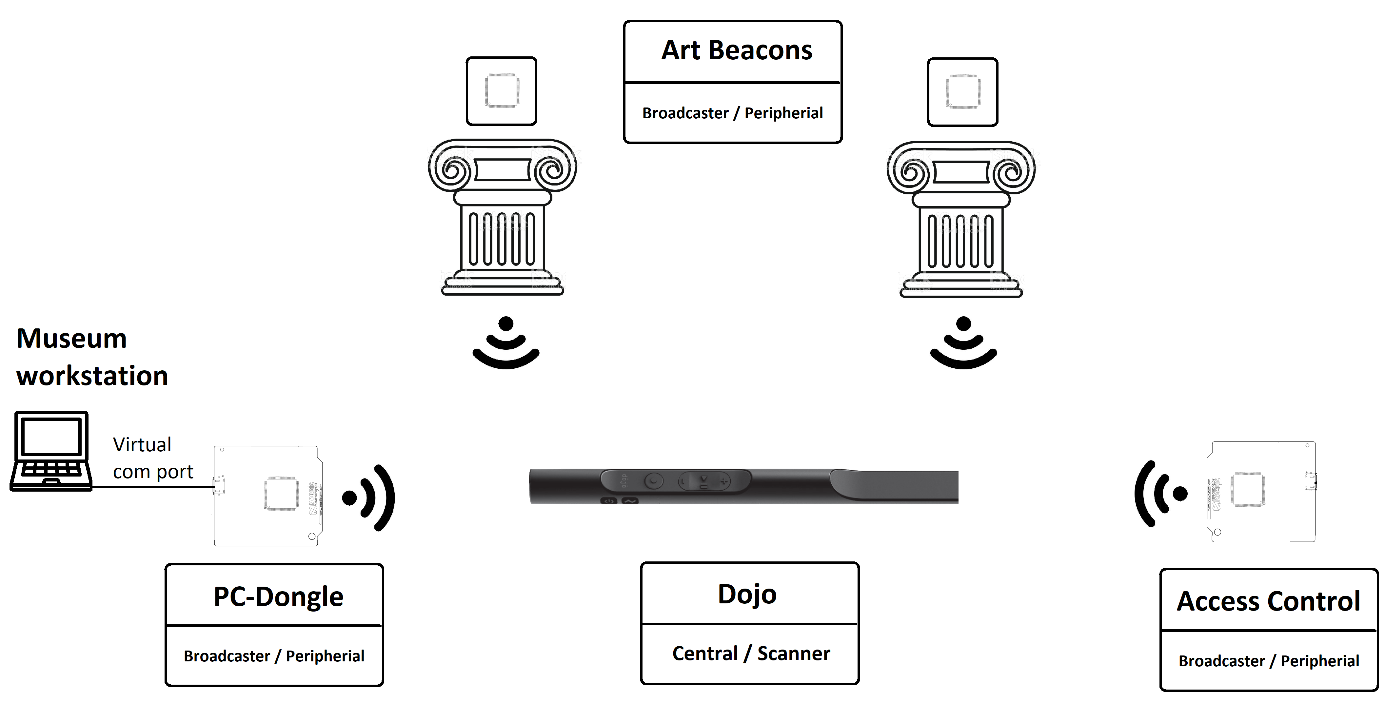
\includegraphics[width=\textwidth]{graphics/platzhalter.png}
	\caption{Museumsumgebung aus Sicht von Bluetooth Low Energy}
	\label{fig:soft_1}
\end{figure}
Die Implementation der in Tabelle \ref{tab:BLE} erwähnten Profile werden nachfolgend beschrieben. 
Auf dem Link-Layer implementieren die Peripheriegeräte einen Advertiser. Dieser sendet periodisch Datenpakete an die Umwelt. Der Inhalt wurde dabei auf ein Minimum beschränkt. Ausgesendet wird nur die Peer-Adresse ohne Payload. Mit einem Flag wird zusätzlich signalisiert, 
dass es sich um ein ''non discoverable'' device handelt. 
Damit wird verhindert, dass fremde Geräte (z.B. Mobiltelefone) beim Scannen der Umgebung die Peripheriegeräte des Museums 
finden können. 
Natürlich können die Geräte mit einer entsprechenden Software trotzdem gefunden werden. Sie werden nur standardmässig nicht angezeigt.
Es ist jedoch trotzdem möglich, bei Kenntnis der Geräteadresse eine Verbindung auszubauen. Dies wurde im Projekt auch so verwendet (Erläuterung erfolgt später).
Auf GAP-Ebene sind alle Parameter für den Verbindungsaufbau hinterlegt. Zusätzlich wird auf der Seite des \textit{Central Devices} eine Whitelist implementiert. Diese sorgt dafür, dass beim Scannen nur die Geräte gefunden werden, welche auch zum Museum gehören.
Als eigentliche Anwendung wurde ein UART-Service auf GATT-Ebene implementiert, der sogenannte NUS (Nordic UART Service). Dieser ermöglicht die Kommunikation zwischen den Geräten. Alle Benutzerdaten, welche über BLE übertragen werden, können bei Bedarf direkt auf die interne UART-Schnittstelle umgeleitet werden. Die Kommunikation von Dojo zu PC-Dongle zur Java-Applikation wurde auf diese Weise realisiert.

\subsubsection{Softwaremässiger Aufbau der Bluetooth-Kommunikation}
Alle oben beschriebenen Vorgänge werden vom sogenannten \textit{Softdevice} von Nordic Semiconductors übernommen. Dabei handelt es sich um eine Firmware, welche vor dem Flashen der eigentlichen Software auf die CPU geladen wird. Dieses stellt alle notwendigen Funktionen zur Verfügung, um Profile und dazugehörige Handler zu initialisieren. Für jedes Profil wird eine Instanz erstellt, welche das Softdevice periodisch im Hintergrund abarbeitet. 
Das für das Projekt entwickelte Bluetooth Softwaremodul hat nun die Aufgabe, alle Instanzen mit den korrekten Parametern zu initialisieren und alle Ereignisse der Handler korrekt zu verarbeiten. Die Softwarestruktur folgt dabei dem hierarchischen Ansatz von BLE. Für jede Abstraktionsebene gibt es einen dazugehörigen Handler. An dieser Stelle sei noch angemerkt, dass das Softdevice in der Handhabung nicht zwischen dem Link-Layer und dem GAP-Layer unterscheidet.
Wie bereits erwähnt, können Verbindungen nur bei bekannter Geräteadresse aufgebaut werden. D.h. allen Geräten wurde eine fixe Adresse zugewiesen. Die Struktur der Adressvergabe ist in Tabelle \ref{tab:BLE_Adresse} ersichtlich.
\begin{table}[h]
  \centering
  \begin{tabular}{|c|c|c|c|c|c|c|}
    \hline
      & \textbf{Byte 0} & \textbf{Byte 1} & \textbf{Byte 2} & \textbf{Byte 3} & \textbf{Byte 4} & \textbf{Byte 5}\\
    \hline
    \textbf{Dojo} 			& 0xFF & 0x13 & 0x37 & 0x13 & 0x37 & 0xFF \\
    \hline
    \textbf{PC Dongle} 			& 0xFF & 0x13 & 0x37 & 0x42 & 0x69 & 0xFF \\
    \hline
    \textbf{Zugangskontorlle 1} 	& 0xFF & 0x13 & 0x37 & 0x0C & 0x01 & 0xFF \\
    \hline
    \textbf{Zugangskontorlle 2} 	& 0xFF & 0x13 & 0x37 & 0x0C & 0x02 & 0xFF \\
    \hline
    \textbf{Zugangskontorlle 3} 	& 0xFF & 0x13 & 0x37 & 0x0C & 0x03 & 0xFF \\
    \hline
    \textbf{ ... } 			& 0xFF & 0x13 & 0x37 & 0x0C & ...  & 0xFF \\
    \hline
    \textbf{Kunstwerkbeacon 1} 		& 0xFF & 0x13 & 0x37 & 0x00 & 0x01 & 0xFF \\
    \hline
    \textbf{Kunstwerkbeacon 2} 		& 0xFF & 0x13 & 0x37 & 0x00 & 0x02 & 0xFF \\
    \hline
    \textbf{Kunstwerkbeacon 3} 		& 0xFF & 0x13 & 0x37 & 0x00 & 0x03 & 0xFF \\
    \hline
    \textbf{ ... } 			& 0xFF & 0x13 & 0x37 & 0x00 & ...  & 0xFF \\
    \hline
  \end{tabular}
  \caption{Adressverteilung der BLE-Geräte}\label{tab:BLE_Adresse}
\end{table}
\vspace{1cm}
\paragraph{Anmerkung: }Der BLE-Standard definiert verschiedene Typen von Adressen und bestimmt Rahmenbedingungen für dessen Aufbau (siehe Core v5.0 Seite 2557 \cite{BLE_SPEC} für genauere Details). Unsere Geräte verwenden sogenannte \textit{random static device addresses}.
Der Gewinn dieser Adressvergabe liegt darin, dass beim Scannen nur wenige Bytes ausgewertet werden müssen, um zu erkennen, um welche Art von Gerät es sich handelt.
Der Nachteil dieses Konzepts ist die schlechte bzw. nicht vorhandene Konvergenz. BLE Geräte arbeiten normalerweise mit zufällig generierten Adressen sowie auf der Basis einer Whitelist. Ein Scanner sucht bei Peripheriegeräten nach sogenannten Service IDs (uuid). Ist diese gefunden, so gehört das Gerät zum System und er schreibt die dazugehörige Geräteadresse in die Whitelist. Aus Performancegründen wurde auf dieses Vorgehen verzichtet, da der Dojo möglichst schnell möglichst viele Adressen scannen und auswerten soll. Da die Gesamtgrösse des Systems durch die Hardware begrenzt ist (Audiochip bzw. bei sehr grossen Audiodateien spätestens durch den Speicher), spielt dieser Faktor keine bedeutende Rolle. 
\vspace{1cm}


Alle weiteren Erläuterungen über das Bluetooth-Modul und dessen genauen Ablauf werden in den dazugehörigen Kapiteln erklärt. Diese Einführung diente dazu, sich einen Überblick über das System zu schaffen und einige wichtige Begriffe zu erläutern, damit die Beschreibung des Programmablaufs besser verständlich wird. 

\subsection{Firmware des Dojos}
Die Firmware des Dojos bildet den grössten Teil der Softwareentwicklung und ist dementsprechend etwas umfangreicher, da das gesamte Management der Bluetooth-Kommunikation sowie der Programmablaufsteuerung darin implementiert wurde. Das Konzept zielt darauf, dass der Dojo möglichst "intelligent" ist, und die Peripheriegeräte möglichst "unintelligent" sind. 
Zuerst wird kurz erläutert, was die Software alles können soll, also wie der Ablauf aus nicht technischer Sicht aussieht. Danach wird das grundlegende Konzept der Implementation erläutert. Zuletzt der genaue Programmablauf eines jeden Teils beschrieben und somit auch die detaillierte Implementation aller Anforderungen.
\subsubsection{Anforderungen an die Software}
Im Normalbetrieb scannt die Software periodisch nach Peripheriegeräten. Immer dann, wenn der Besucher in der Nähe eines Bacons steht, benachrichtigt er diesen durch eine kurze Vibration. Die Auswertung muss dabei so intelligent sein, dass in Grenzfällen keine permanenten Notifikationen ausgesendet werden. Beim Drücken der Play-Taste ladet der Dojo die zum Beacon gehörende Audiodatei und spielt diese ab. Um dies zu bewerkstelligen, müssen die Beacon-IDs mit den Audiodateien verknüpft werden. 
Die genaue Logik beim Museumsrundgang wurde in Zusammenarbeit mit der Auftraggeberin entwickelt. (Was passiert, wenn der Benutzer zu einem neuen Beacon läuft, während eine Wiedergabe läuft? Wird beim Pausieren und anschliessenden Fortsetzen die neue Audiodatei geladen, falls sich der Besucher in dieser Zeit fortbewegt hat? Usw.) Diese Fragen sind im Anhang \ref{Briefverkehr mit Auftraggeberin} dokumentiert.
Neben dem Normalbetrieb gibt es zwei Spezialfälle. Erstens die Zutrittskontrollstationen. Hält der Benutzer seinen Dojo an solch eine Station, so muss die Software diese erkennen, automatisch eine 
Verbindung aufbauen und die Zutrittsberechtigungen austauschen, gefolgt vom Verbindungsabbau. Hier werden diverse Sicherheitsmechanismen benötigt, im Falle, dass der Datenaustausch nicht erfolgreich ist oder sonstige Probleme auftreten (z.B. wenn der Besucher vorzeitig davonläuft). 
Der zweite Spezialfall ist das Konfigurieren des Dojos am Computer der Museumsmitarbeiter. Wann soll der Normalbetrieb wieder aufgenommen werden, wenn keine Daten empfangen werden? Der Dojo muss schliesslich auf Befehle der Java-Software warten. Was wenn die Übertragung nicht vollständig war? Wann werden Daten übernommen, wann werden sie verworfen? Auch hier sind einige Sicherheitsmechanismen notwendig.
\subsubsection{Konzept des Hauptprogrammablaufs}
Das Gesamtkonzept der Firmware basiert auf einem Mix zwischen interruptgesteuerten Statemachine und Verarbeitung von Interruptereignissen im Hauptprogramm. Die Software besitzt sechs Hauptzustände. 
\begin{table}[h]
  \centering
  \begin{tabular}{|p{4cm}|p{11cm}|}
    \hline
    Idle Mode & Der Dojo scannt nach Beacons und benachrichtigt den Benutzer über dessen Dasein.\\
    \hline
    Play Mode & Der Dojo spielt zurzeit eine Audiodatei ab. Das Scannen und Auswerten von Beacons läuft normal im Hintergrund weiter. \\
    \hline
    Pause Mode & Eine Wiedergabe wurde pausiert. Der Scanvorgang läuft auch hier weiter. \\
    \hline
    Like Mode & Der Benutzer hat die Like-Taste betätigt. Das Scannen wird kurzzeitig pausiert und eine Verbindung zum Beacon aufgebaut. Dieser Zustand wird nach kurzer Zeit selbstständig wieder verlassen. \\
    \hline
    Door Control Mode & Der Dojo befindet sich sehr nahe an einer Zugangskontrollstation. Er muss nun selbstständig seine Berechtigungen mit dieser austauschen und danach den Normalbetrieb fortsetzen. \\
    \hline
    PC Connection Mode & Der Dojo befindet sich sehr nahe am PC-Dongle. Er wartet auf dessen Konfigurationsbefehle. Nach erfolgreicher Übertragung wird der Normalbetrieb wieder aufgenommen.\\
    \hline
  \end{tabular}
  \caption{Hauptzustände des Hauptprogrammablaufs}\label{tab:BLE_2}
\end{table}

Während des Abarbeitens der States können sehr viele Ereignisse auftreten. Diese werten unterteilt in kritische und unkritische Ereignisse. Damit ist vorwiegend deren Einfluss auf den Programmablauf gemeint und nicht deren Dringlichkeit. 
Unkritische Ereignisse haben keinen wesentlichen Einfluss auf den Programmablauf und werden sofort in der Interruptroutine abgearbeitet. Dazu gehören die Lautstärke +/- Taste und die Signalisation vom Softdevice, dass ein Advertisement Paket empfangen wurde (BLE Advertisement Event).
Alle anderen Ereignisse sind kritisch und setzen nur Eventflags. Diese werden erst im Hauptprogramm verarbeitet, da sie nur unter bestimmten Bedingungen ausgeführt werden dürfen. Abbildung \ref{Softwarekonzeptzeichnung2.pdf} zeigt eine Übersicht über den Programmablauf. \\

An dieser Stelle sollte kurz geklärt werden, weshalb ''kritische'' Ereignisse nur im Mainloop verarbeitet werden.
Grundsätzlich sind alle Events, welche BLE-Funktionen des Softdevices auslösen, problematisch. Das Softdevice deaktiviert für die Dauer der Ausführung alle Interrupts. Dies ist weniger das Problem, da ansonsten keine zeitkritischen Vorgänge abgearbeitet werden müssen. Problematisch ist das Ausführen von BLE Funktionen zu falschen Zeitpunkten. Dies führt nämlich zum Absturz der Software. Für eine sichere Verwendung unterstützt das Softdevice ein Error-Handling. D.h. alle Funktionen können Fehlercodes zurückgeben, welche ausgewertet werden können. Diese sind jedoch sehr beschränkt und lassen oft keine eindeutige Identifikation des Fehlers zu. Aus diesem Grund entschieden wird uns für einen anderen Ansatz. Alle kritischen Funktionen können nur im Hauptprogramm verarbeitet werden. Dieses sorgt durch intelligente Steuerung des Ablaufs sowie durch Signalisieren von Flags dazu, dass das Programm zuverlässig läuft und BLE-Funktionen nie ''zum falschen Zeitpunkt'' aufgerufen werden können. Das Error Handling dient lediglich zur Verifikation des Ablaufs.
Einzige Ausnahme ist das ''order received'' Ereignis, welches ein Kommunikationsprotokoll übersetzt (Erklärung später). Das Verarbeiten von Strings dauert zu lange für eine ISR und ist deshalb ausgelagert.
Nun sind die Anforderungen und der Aufbau der Software bekannt. Nachfolgend ist die ausführliche Implementierung der Hauptzustände dokumentiert. Anschliessend erfolgt noch ein Kapitel über die Ansteuerung der verbauten Hardware des Dojos.

\subsubsection{Verhalten während des Museumsrundgangs}
Die Modi Idle Mode, Play Mode und Paus Mode sind das, was zuvor als Normalzustand betitelt wurde. Die meiste Zeit über wird sich der Dojo in diesen drei Zuständen befinden.
In allen drei Zuständen wird kontinuierlich nach Beacons gescannt. Dieser Vorgang wird durch einen Timer gesteuert. Das Hauptprogramm aktiviert den Scanvorgang und startet den Timer. Während des Scanvorgangs löst das Softdevice sogenannte Advertisement Events aus.\\ Dies ist immer dann der Fall, wenn ein Paket empfangen wurde. Der dazugehörige Handler prüft anschliessend, ob die Adresse zum System gehört. Falls dem so ist, so wird überprüft, um welche Art von Peripheriegerät es sich handelt. Gehört die Adresse zu einem Beacon, so wird sie zusammen mit dem gemessenen RSSI-Wert (Signalstärke) in einem Buffer abgelegt. Nach 1 Sekunde wird der Timer auslösen und das Scannen wieder beenden. Nun wird der Inhalt des Buffers evaluiert. Es wird nach dem stärksten Beacon (höchster RSSI Wert) gesucht. Dessen Adresse, RSSI-Wert sowie interne ID werden global gespeichert.\\ Zu jeder Adresse ist eine ID verknüpft. Diese ID dient einerseits dem Benutzer als Kennungsmarke für das Aufsetzen einer Ausstellung mit der PC-Applikation, andererseits erlaubt sie eine effiziente Verarbeitung innerhalb der Software, da nur eine 8-Bit lange ID anstatt einer 48-Bit-Adresse gearbeitet werden kann.
In der Statemachine, d.h. in einem der drei genannten Zuständen, wird die zuvor evaluierte Adresse mit dem stärksten Beacon des vorherigen Scanvorgangs verglichen. Der Vergleich nach jedem Timerintervall zwischen ''neuer stärksten Adresse'' und ''vorheriger stärksten Adresse'' bildet den Grundsatz für die Steuerung des Hauptprogramms. Immer dann, wenn fünf Mal hintereinander die ''neue stärkste Adresse'' ungleich der aktuellen ist, wird der Benutzer durch Vibration notifiziert und die ''vorherige stärkste Adresse'' wird durch die neue ersetzt. (Bei den fünf Mal handelt es sich um einen Erfahrungswert, welcher gut funktionierte).\\
Was passiert, wenn gar kein Beacon gefunden wurde? \\In diesem Fall liefert die Evaluation des Buffers eine Adresse aus lauter Nullen zurück. Diese wird trotzdem ausgewertet und gegebenenfalls gespeichert. Dies ist notwendig, damit die Software weiss, dass der Benutzer ''davongelaufen'' ist. Damit wird verhindert, dass beim Drücken der Play- oder Like-Taste versucht wird, sich mit einem Beacon zu verbinden, welcher schon lange ausser Reichweite ist.
Des Weiteren ist eine minimale Signalstärke definiert. Nur wenn die Signalstärke grösser als dieser Wert ist, wird die Adresse gebuffert. Damit wird verhindert, dass der Benutzer notifiziert wird, falls er sehr weit von sämtlichen Beacons entfernt ist.
Nach dem Auswerten des Buffers wird dieser gelöscht und der Vorgang startet von Neuem. Einen Wechsel in den Play Mode erfolgt dann, wenn der Benutzer die Play/Pause-Taste betätigt. Diese ist so konfiguriert, dass sie bei jedem Tastendruck eine Variable toggelt. Ob die Variable getoggelt wurde, wird in jedem Durchgang gepollt. Die genaue Auswirkung ist vom Zustand des Programms abhängig. Ist das Programm im Idle Mode, so erfolgt der Wechsel in den Play Mode.\\
In diesem Zustand wird zuerst geprüft, ob der aktuell gespeicherte stärkste Beacon keine ''Nulleradresse'' ist. Falls dies nicht der Fall ist, so wird das zum Beacon gehörende Audiostück mit der konfigurierten Sprache abgespielt. Anderenfalls wechselt das Programm sogleich in den Idle Zustand zurück. Wie die Beacon-IDs mit den Audiodateien verknüpft sind, wird in Kapitel \ref{Softwarekonzeptzeichnung3.pdf} erklärt.
Solange eine Audiodatei wiedergegeben wird, erfolgt das Scannen und Baffern von Beacons auf gleiche Weise wie im Idle Mode.\\\\
Allerdings gibt es zwei Spezialfälle. Im ersten Fall hört sich der Benutzer das Stück komplett an, bis es zu Ende ist. Der verwendete Audiochip kann dies signalisieren. Der Status vom Audioplayer wird ebenfalls bei jedem Durchgang geprüft. Ist dies der Fall, so wird das Programm zurück in den Idle Mode wechseln. Im zweiten Spezialfall entfernt sich der Benutzer, während die Wiedergabe läuft. D.h. es wurde fünfmal hintereinander eine neue stärkste Adresse lokalisiert.\\ Dem Programm wird nun signalisiert, dass sich der Benutzer vor einem neuen Ausstellungsstück befindet. Nun kommt die bereits erwähnte Logik zum Einsatz. Die Auftraggeberin wünschte, dass in diesem Fall ebenfalls ein Feedback an den Benutzer gesendet wird (Vibration). Bei einem Drücken der Play-Taste wird nun die Audiodatei des neuen Beacons geladen.\\
Der letzte Zustand im Normalmodus ist der Pause Mode. Wie der Name vermuten lässt, landet das Programm immer hier, wenn die Play/Pause-Taste während einer Wiedergabe gedrückt wurde. Das Verhalten ist äquivalent zum Play Mode. Das Scannen wird fortgesetzt und der Benutzer wird benachrichtigt, wenn er davonläuft und ein neuer Beacon der stärkste wird. Die Logik wurde hier so implementiert, dass bei einem Tastendruck das alte Audiostück nicht fortgesetzt wird, sondern ebenfalls das neue geladen wird. 
Der gesamte Ablauf dieser drei Modi ist in der Abbildung \ref{Softwarekonzeptzeichnung3.pdf} graphisch abgebildet.\\
 
 
Abschliessend zu den drei Normalzuständen noch ein paar allgemeine Informationen: Bei jedem Wechsel des stärksten Beacons wird ein zusätzlicher Timer, Beacon Switch Timer genannt, gestartet. Dieser signalisiert mit einem Flag, dass zurzeit kein Wechsel des stärksten Beacon möglich ist. Immer dann, wenn nach der Evaluation des Buffers kein neuer stärkster Beacon gefunden wurde, wird der RSSI-Wert des vorherigen stärksten Beacons aktualisiert. Damit trackt das Programm die aktuelle Signalstärke des Beacons. Diese Information ist für den Like Mode von Bedeutung, welcher nachfolgend dokumentiert wird.
\subsubsection{Liken von Ausstellungsstücken}
Die Aufgabe des Like Mode ist schnell erklärt. Der Dojo soll eine Verbindung aufbauen, den Beacon über das Liken informieren, anschliessend die Verbindung wieder abbauen und zurück in den Idle Mode gehen.
Drückt der Benutzer die Like-Taste, so wird zuerst das Scannen unterbrochen und geprüft, ob nicht schon eine Verbindung vorhanden ist und ob der aktuell stärkste Beacon keine Nulleradresse ist. Ist der stärkste Beacon eine gültige Adresse, so wird dessen ID gespeichert und zusätzlich geprüft, ob die Signalstärke eine vordefinierte Mindeststärke erfüllt. Nur dann wird eine Verbindung aufgebaut. Wie bereits erwähnt, wechselt der stärkste Beacon nur dann, wenn dieser fünfmal hintereinander als stärkster Sender evaluiert wurde. Diese Lokalisierung ist also ein wenig träge. Aus diesem Grund wird die Signalstärke kontinuierlich aktualisiert, damit bei einem Davonlaufen nicht versucht wird, eine Verbindung zu einem eventuell zu weit entfernten Beacon aufzubauen.
Nun zum eigentlichen Verbindungsauf- und Abbau. Als Erstes wird versucht, eine Verbindung aufzubauen. Das Programm wartet dabei auf das BLE GAP Connected Event. Dieses signalisiert, dass die Verbingung nun etabliert ist. Der Dojo sendet nun eine kurze Nachricht an den Beacon und wartet auf eine Quittierung. Danach wird die Verbindung abgebaut und auf das BLE GAP Disconnected Event gewartet. Hat alles geklappt, so wechselt die Software in den Idle Mode und nimmt den Normalbetrieb wieder auf. Damit die Software nicht hängen bleibt, z.B. weil die Daten nicht empfangen wurden oder weil die Verbindung nicht zu Stande kommt, wird bei jedem versuchten Verbindungsaufbau ein Timeout-Timer gestartet. Bei einer erfolgreichen Übertragung wird dieser vorzeitig gestoppt. Anderenfalls sorgt das Auslösen des Timers dafür, dass die Verbindung abgebrochen und das Programm fortgesetzt wird. Der Benutzer muss in diesem Fall die Like-Taste für einen erneuten Versuch nochmals betätigen. Abbildung \ref{Softwarekonzeptzeichnung3.pdf} zeigt das Ablaufdiagramm des Like Mode.
\subsubsection{Datenaustausch mit Zutrittskontrollstationen}
Eine weitere Funktion der Software ist das automatisierte Austauschen von Zutrittsrechten. Beim Scannen prüft der Handler, von welchem Gerät das Datenpaket stammt. Gehört das Paket zu einer Zutrittskontrollstation, so wird überprüft, ob die Signalstärke grösser als -35dB ist. Dies entspricht wenigen Zentimetern Distanz zwischen Dojo und Sender. In diesem Fall wird dem Hauptprogramm ein ''Door Control Request'' signalisiert. Der restliche Ablauf ist nun sehr ähnlich zum Like Mode (Prüfen von Flags, starten des Timeout-Timers). Der einzige Unterschied besteht darin, dass bei einem erfolgreichen Abschliessen ein weiterer Timer gestartet wird, der No connection Timer. Dieser verhindert, dass das Programm nach dem Verbindungsabbau gleich wieder versucht, eine neue Verbindung aufzubauen, sollte der Besucher den Dojo immer noch nahe an der Station halten.
Für den eigentlichen Datenaustausch wurde ein kleines Kommunikationsprotokoll entwickelt. Die genaue Funktionsweise und Implementierung in der Software ist im Anhang \ref{Softwarekonzeptzeichnung3.pdf} zu finden. Dieses wird für die Kommunikation mit allen Peripheriegeräten genutzt. 
Die Zutrittsberechtigungen sind sehr einfach implementiert worden, um dessen Funktionsweise konzeptionell zu demonstrieren. Alle benutzerspezifischen Daten (Sprache, Zutrittsrechte sowie der Speicher für die gelikten Beadon-IDs) sind in einem globalen Struct hinterlegt. Die Zutrittsrechte sind in einer 32Bit Variable hinterlegt, wobei jedes Bit die Rechte eines Sektors repräsentiert (1 = Zutritt, 0 = kein Zutritt). Bei der Konfiguration des Dojos werden die entsprechenden Berechtigungen einfach auf diese Variable aufmaskiert. In einer tatsächlichen Realisierung des Projekts müsste man an dieser Stelle einige Sicherheitsfeatures implementieren (Keys für Zutrittsrecht, evt. sogar eine Verschlüsselung), damit das digitale Ticket auch sicher ist.
Auf ein Diagramm wird an dieser Stelle verzichtet, da mit Ausnahme des Datenaustausches das Vorgehen praktisch gleich ist wie im Like Mode.

\newpage

\subsubsection{Konfiguration und Auswertung des Dojos}
Der letzte Hauptzustand ist der PC Connection Mode . Der Verbindungsaufbau erfolgt gleich wie im Door Control Mode. Ist der Dojo sehr nahe am Dongle, so wird die Verbindung geöffnet. Die Software wartet nun auf Anweisungen von der Java-Software. Dies ist die einzige Verbindung, bei welcher kein Timeout-Timer gestartet wird, da es nicht vorhersehbar ist, wie lange der Dojo beim Personal liegt und konfiguriert wird. Damit das Programm nicht bis in alle Ewigkeit auf Anweisungen wartet, wird mit jedem Durchgang geprüft, ob die Verbindung noch steht. Ist dies nicht der Fall, so wird der Dojo wieder in den normalen Betriebszustand einnehmen. 
Steht die Verbindung so, wartet der Dojo auf zwei Befehle. Entweder will das Personal die Daten auswerten, d.h. die IDs der gelikten Beacons auslesen, oder der Dojo soll neu konfiguriert werden. Im ersten Fall wird die Software alle IDs übertragen und nach einer Quittierung den Speicher löschen und die Verbindung trennen. Möchte man den Dojo nach der Auswertung neu konfigurieren so muss das Personal kurz warten bis der No connection Timer abgelaufen ist. Bei einer Konfiguration werden sequenziell die Zugriffsrechte und die gewünschte Sprache übertragen. Die Linkinformationen für Beacon ID und dazugehörige Audiodatei müssen nicht übertragen werden. Diese kann sich der Dojo dank intelligenter Namensgebung errechnen (siehe Kapiel \ref{fig:soft_6}). Wichtig ist, dass der Dojo vorhergehende Zugriffsrechte nicht löscht. Damit erhält man die Möglichkeit, während des Besuchs weitere Ausstellungen zu erschliessen. Eine Löschung erfolgt also erst dann, wenn die gelikten IDs übertragen wurden.

\newpage

\subsubsection{Ansteuerung der Hardware }
In den Abbildungen \ref{Softwarekonzeptzeichnung3.pdf} sind noch nicht alle einzelnen Punkte erläutert worden. Was bisher ausgelassen wurde, ist die Ansteuerung der Hardware. Damit der Dojo mit seiner Umwelt agieren kann, wird diverse Peripherie benötigt (nicht zu Verwechseln mit den Bluetooth Peripheriegeräten). Als Peripherie werden alle Aktoren betrachtet, welche auf dem Dojo angebracht sind. Dieses Kapitel erläutert die wichtigsten Zusammenhänge der einzelnen Peripherieeinheiten. Abbildung \ref{fig:p_uebersicht} zeigt die Verbindungen zwischen den einzelnen Komponenten.
\begin{figure}[htb]
\begin{center}
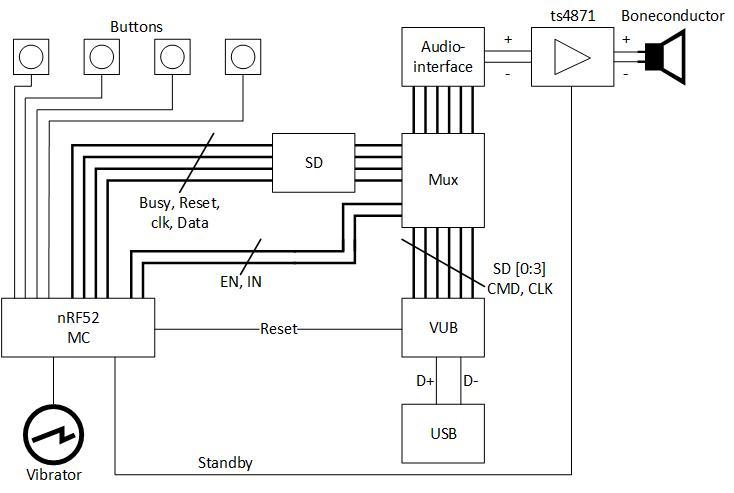
\includegraphics[width=\textwidth]{periphery_uebersicht.jpg}
\caption{Übersicht Periphery} % picture caption
\label{fig:p_uebersicht}
\end{center}
\end{figure}
Das Abspielen von Audiodateien wird vom Audiochip wtv020sd gesteuert. Dieser wiederum steuert das Audiointerface, welches die Daten von der SD-Karte liest. Die Kommunikation zum Audiochip erfolgt via SPI-Schnittstelle. Die Daten werden als 16-Bit-Befehle übertragen. Die genaue Codierung kann aus dem Datenblatt entnommen werden [QUELLE]. Um den Chip zurückzusetzen oder den Status abzufragen reicht das Setzen bzw. Auslesen eines GPIO-Pins (General Purpose Input Output). Das Audiointerface kann die Audiodaten abspielen, pausieren, stoppen sowie die Lautstärke vermindern oder erhöhen. 
Ebenfalls durch Setzen von GPIO-Pins können der Audioverstärker ein- und ausgeschalt, der Vibrator gestartet oder gestoppt sowie der Multiplexer umgeschaltet werden. Es wird zwischen Audio- und USB-Modus unterschieden. Jeweils nur eines der beiden Geräte kann auf die SD-Karte zugreifen. Für die Software bedeutet dies, dass bei der Verbindung zum PC-Dongle auf USB-Modus gewechselt werden muss, damit die Java-Applikation auf die SD-Karte zugreifen kann. Für den restlichen Betrieb befindet sich der Multiplexer im Audio-Modus.
\subsection{Firmware der Peripheriegeräte}
Nicht nur der Dojo benötigt eine Software, sondern auch die ganzen Bluetooth Peripheriegeräte. Alle drei Typen (Beacon, PC-Dongle und Zutrittskontrollstation) arbeiten mit dem gleichen Quellcode. Die Unterscheidung des Programmablaufs erfolgt durch das setzen globaler defines im entsprechenden Headerfile. Die Funktionsweise ist schnell erklärt, da die Peripheriegeräte wie bereits erwähnt unintelligent sind und sein sollen. 
Im Wesentlichen senden sie ihre Advertisement-Pakete aus und warten auf Verbindungsanfragen des Dojos. Der Quellcode vom Dojo sowie derjenige der Peripheriegeräte nutzen die gleichen Algorithmen und Bibliotheken. D.h. alle Geräte kennen das Kommunikationsprotokoll sowie die zugewiesenen IDs zu den Geräteadressen. 
Die Beacons und die Zutrittskontrollstationen machen nichts Weiteres, als auf Anfragen des Protokolls zu antworten und empfangene Daten zu quittieren. Der PC-Dongle wertet die empfangenen Daten nicht aus, sondern sendet sie an die PC-Applikation. Damit wäre die Funktionsweise aller Peripheriegeräte bereits erklärt.
\subsection{PC-Applikation}
Um es dem Benutzer so einfach wie möglich zu machen, wurde eine Java Anwendung gestaltet, welche Audiodateien korrekt auf den Dojo übertragen, ihn konfigurieren sowie dessen Daten (gelikte Beacon IDs) auslesen kann.
Für den Zugriff auf die SD-Karte wird diese durch den Multiplexer im Prinzip als normaler Wechseldatenträger eingebunden. Die Applikation erkennt dies und kopiert die Audiodateien ''ganz normal'' auf die SD-Karte. Die Besonderheit liegt in der Namensgebung. Der Benutzer wählt aus, welche Audiodatei zu welcher Beacon-ID gehört. Dabei handelt es sich um dieselben IDs, wie sie der Dojo und die Peripheriegeräte intern nutzen. Da sich alle Audiodateien für alle Sprachen gleichzeitig auf dem Dojo befinden, wird diese Information ebenfalls in die Namensgebung hineincodiert. Die Codierung ist in Abbildung \ref{fig:soft_5} zu sehen.
\begin{figure}[h]
	\centering
	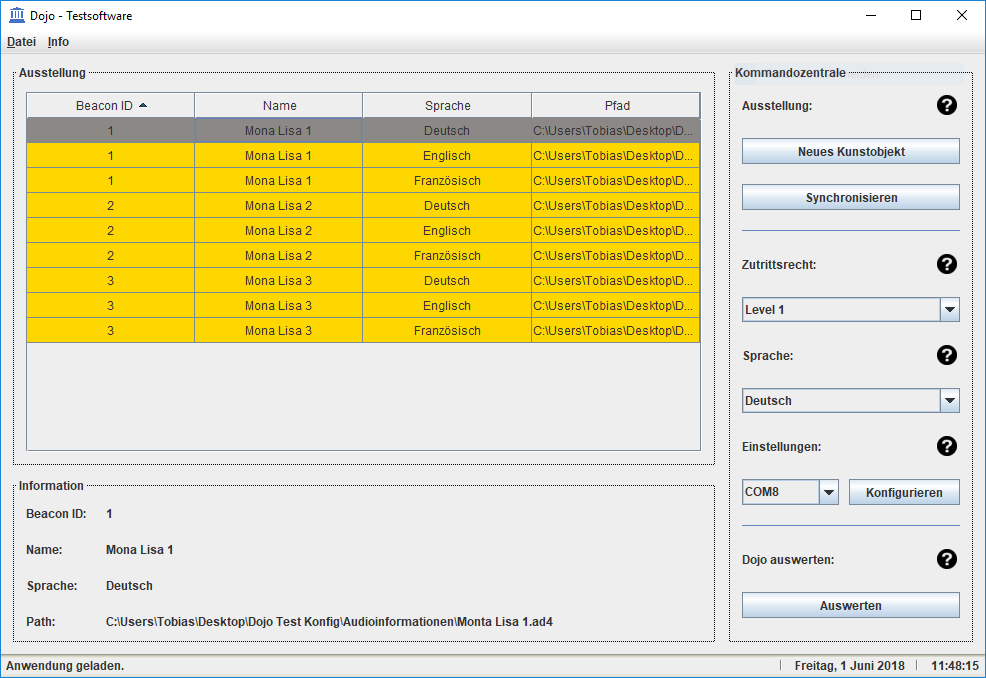
\includegraphics[width=\textwidth]{graphics/Java_Anwendung.png}
	\caption{Java Anwendung}
	\label{fig:soft_5}
\end{figure}
Um die korrekte Audiodatei zu ermitteln muss, der Dojo also lediglich die Beacon ID mal 10 rechnen und die Sprache dazu addieren. Somit spart man sich das Übertragen einer gegebenenfalls sehr langen Liste von Beacon-IDs und Audiodateinamen.
Im Gegensatz zu den Audiodateien werden die Konfigurationsinformationen sowie das Auslesen der gelikten Beacons drahtlos über BLE übertragen. Diese Aufgabe übernimmt der PC-Dongle. Die Befehle müssen aber zuerst auf diesen gelangen. Zwischen Dongle und PC wird eine virtuelle serielle Schnittstelle emuliert, über welche die Kommunikation läuft. Aus diesem Grund muss der Benutzer den entsprechenden COM-Port im Programm selektieren. Natürlich bedingt besagter Vorgang auch, dass der Dojo nahe beim Dongle ist. \newpage
Als letzte Funktion wird das Aufsetzen einer Ausstellung erläutert. Abbildung \ref{fig:soft_6} zeigt die Java- Anwendung, in der zurzeit gerade eine Ausstellung mit drei Kunstobjekten (in allen drei Sprachen) geladen ist. Per ''Neues Kunstobjekt'' kann er eine Audiodatei einer Beacon-ID zuweisen. Statusmeldungen sowie eventuelle Fehleingaben werden in der Statusleiste unten links ausgegeben.
\begin{figure}[h]
	\centering
	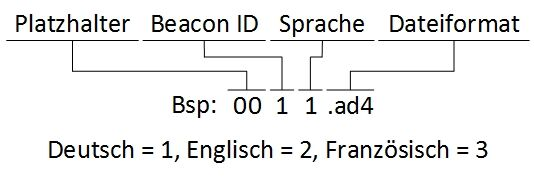
\includegraphics[width=10cm]{graphics/Dateiname_Konvention.jpeg}
	\caption{Dateiname Konventionen}
	\label{fig:soft_6}
\end{figure}

\newpage

\subsection{Softwarelizenzen}
Die in diesem Projekt entwickelte Hard- und Software wird unter den Bedingungen der GNU
GPL v3 (GNU General Public License) freigeben. Das komplette Softdevice S132 Version 5.1.0,
sowie die SDK v14.2 (Software Development Kit), welche für die Erstellung der Firmware verwen-
det wurde, steht dabei unter Lizenz von Nordic. Zudem steht die in Java verwendete Bibliothek
simple-xml-2.7.1 unter Lizenz von Apache, sowie die Bibliothek jSSC-2.7.0-Release unter Lizenz
von GNU GPL v3.
Die originalen Lizenztexte der oben genannten Lizenzen werden im Anhang nicht aufgelistet, da einzelne Lizenzen über 16 Seiten lang sind. Die einzelnen Lizenztexte finden sich im Internet.

\clearpage










%%%%%%%%%%%%%%%%%%%%%%%%%%%%%%%%%%%%%%%%%%%%%%%%%%%%%%%%%%%%%%%%%%%%%%%%%%%%%

%%%%%%%%%%%%%%%%%%%%%%%%%%%%%%%%%%%%%%%%%%%%%%%%%%%%%%%%%%%%%%%%%%%%%%%%%%%%%

